% ------------------------------------------------------------------------
% ------------------------------------------------------------------------
% Modelo UFSC para Trabalhos Academicos (tese de doutorado, dissertação de
% mestrado) utilizando a classe abntex2
%
% Autor: Alisson Lopes Furlani
% 	Modificações:
%	- 27/08/2019: Alisson L. Furlani, add 'glossaries' package
%   - 30/10/2019: Alisson L. Furlani, adjusted some spacing errors and changed math fonts
%   - 17/01/2020: Alisson L. Furlani, updated certification page
%   - 07/02/2020: Alisson L. Furlani, fixed table counter bug
%   - 11/03/2020: Alisson L. Furlani, changed greek letters in math and fixed citation style
% ------------------------------------------------------------------------
% ------------------------------------------------------------------------

\documentclass[
	% -- opções da classe memoir --
	12pt,				% tamanho da fonte
	%openright,			% capítulos começam em pág ímpar (insere página vazia caso preciso)
	oneside,			% para impressão no anverso. Oposto a twoside
	a4paper,			% tamanho do papel. 
	% -- opções da classe abntex2 --
	chapter=TITLE,		% títulos de capítulos convertidos em letras maiúsculas
	section=TITLE,		% títulos de seções convertidos em letras maiúsculas
	%subsection=TITLE,	% títulos de subseções convertidos em letras maiúsculas
	%subsubsection=TITLE,% títulos de subsubseções convertidos em letras maiúsculas
	% -- opções do pacote babel --
	english,			% idioma adicional para hifenização
	%french,				% idioma adicional para hifenização
	%spanish,			% idioma adicional para hifenização
	brazil				% o último idioma é o principal do documento
	]{abntex2}

\usepackage{setup/ufscthesisA4-alf}
\addbibresource{aftertext/references.bib} % Seus arquivos de referências

% ---
% Filtering and Mapping Bibliographies
% ---
\DeclareSourcemap{
	\maps[datatype=bibtex]{
		% remove fields that are always useless
		\map{
			\step[fieldset=abstract, null]
			\step[fieldset=pagetotal, null]
		}
		% remove URLs for types that are primarily printed
%		\map{
%			\pernottype{software}
%			\pernottype{online}
%			\pernottype{report}
%			\pernottype{techreport}
%			\pernottype{standard}
%			\pernottype{manual}
%			\pernottype{misc}
%			\step[fieldset=url, null]
%			\step[fieldset=urldate, null]
%		}
		\map{
			\pertype{inproceedings}
			% remove mostly redundant conference information
			\step[fieldset=venue, null]
			\step[fieldset=eventdate, null]
			\step[fieldset=eventtitle, null]
			% do not show ISBN for proceedings
			\step[fieldset=isbn, null]
			% Citavi bug
			\step[fieldset=volume, null]
		}
	}
}
% ---

% ---
% Informações de dados para CAPA e FOLHA DE ROSTO
% ---
% FIXME Substituir 'Nome completo do autor' pelo seu nome.
\autor{Calil Amaral}

% FIXME Substituir 'Título do trabalho' pelo título da trabalho.
\titulo{
	The effects of wall thickness, overhang angle and curvature radius on the resulting geometry of iron 
	components manufactured by laser directed energy deposition
}
% FIXME Substituir 'Subtítulo (se houver)' pelo subtítulo da trabalho.  
% Caso não tenha substítulo, comente a linha a seguir.
% \subtitulo{subtítulo (se houver)}

% FIXME Substituir 'XXXXXX' pelo nome do seu
% orientador.
\orientador{Prof. Milton Pereira, Dr.}
% FIXME Se for orientado por uma mulher, comente a linha acima e descomente a linha a seguir.
% \orientador[Orientadora]{Nome da orientadora, Dra.}
% FIXME Substituir 'XXXXXX' pelo nome do seu
% coorientador. Caso não tenha coorientador, comente a linha a seguir.
\coorientador{Prof. Walter Lindolfo Weingaertner, Dr.}
% FIXME Se for coorientado por uma mulher, comente a linha acima e descomente a linha a seguir.
% \coorientador[Coorientadora]{XXXXXX, Dra.}
% FIXME Substituir '[ano]' pelo ano (ano) em que seu trabalho foi defendido.
\ano{2022}
% FIXME Substituir '[dia] de [mês] de [ano]' pela data em que ocorreu sua defesa.
%\data{[dia] de [mês] de [ano]}
% FIXME Substituir 'Local' pela cidade em que ocorreu sua defesa.
\local{Florianópolis}
\instituicaosigla{UFSC}
\instituicao{Universidade Federal de Santa Catarina}
% FIXME Substituir 'Dissertação/Tese' pelo tipo de trabalho (Tese, Dissertação). 
\tipotrabalho{Dissertação}
% FIXME Substituir '[mestre/doutor] em XXXXXX' pela grau adequado.
\formacao{mestre em Engenharia Mecânica}
% FIXME Substituir '[mestrado/doutorado]' pelo nivel adequado.
\nivel{mestrado}
% FIXME Substituir 'Programa de Pós-Graduação em XXXXXX' pela curso adequado.
\programa{Programa de Pós-Graduação em Engenharia Mecânica}
% FIXME Substituir 'Campus XXXXXX ou Centro de XXXXXX' pelo campus ou centro adequado.
\centro{Centro Tecnológico}
\preambulo
{%
\imprimirtipotrabalho~submetida~ao~\imprimirprograma~da~\imprimirinstituicao~para~a~obtenção~do~título~de~\imprimirformacao.
}
% ---

% ---
% Configurações de aparência do PDF final
% ---
% alterando o aspecto da cor azul
\definecolor{blue}{RGB}{41,5,195}
% informações do PDF
\makeatletter
\hypersetup{
     	%pagebackref=true,
		pdftitle={\@title}, 
		pdfauthor={\@author},
    	pdfsubject={\imprimirpreambulo},
	    pdfcreator={LaTeX with abnTeX2},
		pdfkeywords={ufsc, latex, abntex2}, 
		colorlinks=true,       		% false: boxed links; true: colored links
    	linkcolor=black,%blue,          	% color of internal links
    	citecolor=black,%blue,        		% color of links to bibliography
    	filecolor=black,%magenta,      		% color of file links
		urlcolor=black,%blue,
		bookmarksdepth=4
}
\makeatother
% ---

% ---
% compila a lista de abreviaturas e siglas e a lista de símbolos
% ---

% Declaração das siglas
\siglalista{ABNT}{Associação Brasileira de Normas Técnicas}

% Declaração dos simbolos
\simbololista{C}{\ensuremath{C}}{Circunferência de um círculo}
\simbololista{pi}{\ensuremath{\pi}}{Número pi} 
\simbololista{r}{\ensuremath{r}}{Raio de um círculo}
\simbololista{A}{\ensuremath{A}}{Área de um círculo}

% compila a lista de abreviaturas e siglas e a lista de símbolos
\makenoidxglossaries 

% ---

% ---
% compila o indice
% ---
\makeindex
% ---

% ----
% Início do documento
% ----
\begin{document}

% Seleciona o idioma do documento (conforme pacotes do babel)
%\selectlanguage{english}
\selectlanguage{brazil}

% Retira espaço extra obsoleto entre as frases.
\frenchspacing

% Espaçamento 1.5 entre linhas
\OnehalfSpacing

% Corrige justificação
%\sloppy

% ----------------------------------------------------------
% ELEMENTOS PRÉ-TEXTUAIS
% ----------------------------------------------------------
% \pretextual %a macro \pretextual é acionado automaticamente no início de \begin{document}
% ---
% Capa, folha de rosto, ficha bibliografica, errata, folha de apróvação
% Dedicatória, agradecimentos, epígrafe, resumos, listas
% ---


% ELEMENTOS PRÉ-TEXTUAIS
\ifforcedinclude\else
    % Fix the \textpreliminarycontents not showing up when @twoside is disabled
    \newif\ifufscThesisXisMemoirTwoSidesEnabled

    % https://tex.stackexchange.com/questions/360785/how-do-i-check-if-a-document-is-oneside-or-twoside
    \ifthenelse{\boolean{@twoside}}{%
        \ufscThesisXisMemoirTwoSidesEnabledtrue%
    }{%
        \ufscThesisXisMemoirTwoSidesEnabledfalse%
    }%
    \setboolean{@twoside}{true}

    % pretextual settings
    % https://tex.stackexchange.com/questions/386446/how-to-fix-destination-with-the-same-identifier-namepage-a-has-been-already
    % https://tex.stackexchange.com/questions/67989/pdftex-warning-has-been-referenced-but-does-not-exist-replaced-by-a-fixed-one
    \hypersetup{pageanchor=false}
    \PRIVATEbookmarkthis{Capa}
    \addtotextpreliminarycontent{Capa}
    \pretextual

    % Capa
    % \includepdf{pictures/FrenteCapaUFSC.pdf}
    % https://tex.stackexchange.com/questions/227711/blank-page-after-titlingpage
    \advisor{}{\AtBeginShipoutNext{\AtBeginShipoutNext{\AtBeginShipoutDiscard}}}
    \imprimircapa

    % https://tex.stackexchange.com/questions/386446/how-to-fix-destination-with-the-same-identifier-namepage-a-has-been-already
    % https://tex.stackexchange.com/questions/67989/pdftex-warning-has-been-referenced-but-does-not-exist-replaced-by-a-fixed-one
    \hypersetup{pageanchor=true}

    % Custom list throw LaTeX Error: Command \mycustomfiction already defined?
    % https://tex.stackexchange.com/questions/388489/custom-list-throw-latex-error-command-mycustomfiction-already-defined/
    \advisor{}{%
        % Manually add the `\textpreliminarycontents` to the Table of Contents here
        % to keep the hyper link pointing to the beginning of the page, instead of
        % the beginning of `\textpreliminarycontents`
        % https://tex.stackexchange.com/questions/44088/when-do-i-need-to-invoke-phantomsection
        \phantomsection\addcontentsline{toc}{chapter}{\mytextpreliminarylistname}

        % https://tex.stackexchange.com/questions/234398/list-of-figures-and-tables-when-there-are-no-figures-or-tables
        \whenlistisnotempty{\mytextpreliminarylistname}{%
            \begin{KeepFromToc}
                \textpreliminarycontents
            \end{KeepFromToc}
        }

        \clearpage
    }

    % Fix the \textpreliminarycontents not showing up when @twoside is disabled
    \ifufscThesisXisMemoirTwoSidesEnabled
        \setboolean{@twoside}{true}
    \else
        \setboolean{@twoside}{false}
    \fi

    % Folha de rosto (o * indica que haverá a ficha bibliográfica)
    % https://tex.stackexchange.com/questions/74439/table-of-contents-incorrect-page-numbering
    \addtotextpreliminarycontent{\folhaderostoname}
    \imprimirfolhaderosto*{}

    % Inserir a ficha bibliografica
    %
    % Isto é um exemplo de Ficha Catalográfica, ou ``Dados internacionais de
    % catalogação-na-publicação''. Você pode utilizar este modelo como referência.
    % Porém, provavelmente a biblioteca da sua universidade lhe fornecerá um PDF
    % com a ficha catalográfica definitiva após a defesa do trabalho. Quando estiver
    % com o documento, salve-o como PDF no diretório do seu projeto e substitua todo
    % o conteúdo de implementação deste arquivo pelo comando abaixo:
    \PRIVATEbookmarkthis{Ficha Catalográfica}
    \addtotextpreliminarycontent{Ficha Catalográfica}

    

\ifenglish

Legal Notes:

There is no warranty for any part of the documented software. The authors have taken care in the
preparation of this thesis, but make no expressed or implied warranty of any kind and assume no
responsibility for errors or omissions. No liability is assumed for incidental or consequential
damages in connection with or arising out of the use of the information or programs contained here.

\else

Notas legais:

Não há garantia para qualquer parte do software documentado. Os autores tomaram cuidado na
preparação desta tese, mas não fazem nenhuma garantia expressa ou implícita de qualquer tipo e não
assumem qualquer responsabilidade por erros ou omissões. Não se assume qualquer responsabilidade por
danos incidentais ou consequentes em conexão ou decorrentes do uso das informações ou programas aqui
contidos.

\fi


% http://portalbu.ufsc.br/ficha
% http://portal.bu.ufsc.br/servicos/ficha-de-identificacao-da-obra/
\begin{fichacatalografica}
    \vspace*{\fill}

    \begin{center}

        \lang
        {Cataloging at source by the University Library of the Federal University of Santa Catarina.}
        {Catalogação na fonte pela Biblioteca Universitária da Universidade Federal de Santa Catarina.}

        \lang
        {File compiled at \currenttime h of the day \today.}
        {Arquivo compilado às \currenttime h do dia \today.}

        \framebox[\textwidth]
        {
            % https://tex.stackexchange.com/questions/369918/use-the-value-of-title-with-removed-linebreak
            \begin{minipage}{0.98\textwidth}
            \begingroup \let\\=\space

                \ttfamily
                \imprimirautor

                \hspace{0.5cm} \imprimirtitulo%
                \ifnotempty{\imprimirsubtitulo}{~:~\imprimirsubtitulo}%
                ~/~\imprimirautor%
                ;~\imprimirorientadorRotulo,~\imprimirorientador%
                \ifnotempty{\imprimircoorientador}{;~\imprimircoorientadorRotulo,~\imprimircoorientador}%
                ~--~\imprimirlocal,~\imprimirdata.

                % Prints how much pages there are on the document and links to the last page
                \hspace{0.5cm} \pageref{LastPage} p.
                \bigskip

                \hspace{0.5cm} \imprimirtipotrabalho~--~\imprimirinstituicao,
                \imprimircentro,~\imprimirprograma.
                \bigskip

                \hspace{0.5cm} \lang{Includes references}{Inclui referências}
                \bigskip

                % https://tex.stackexchange.com/questions/54055/using-lower-case-roman-numerals-in-enumerate-lists
                % https://tex.stackexchange.com/questions/61811/how-to-define-inparaenum-in-the-preamble
                \hspace{0.5cm}
                \begin{inparaenum}
                    \lang{\palavraschaveinglescomvirgula}{\palavraschaveportuguescomvirgula}%
                \end{inparaenum}%
                \begin{inparaenum}[I.]
                    \item \imprimirorientador~
                    \ifnotempty{\imprimircoorientador}{\item \imprimircoorientador~}
                    \item \imprimirprograma~
                    \item \imprimirtitulo~
                \end{inparaenum}%
                \bigskip

                \hspace{7.75cm} CDU 02:141:005.7

            \endgroup
            \end{minipage}
        }

    \end{center}

\end{fichacatalografica}


    % https://tex.stackexchange.com/questions/91440/how-to-include-multiple-pages-in-latex
    % 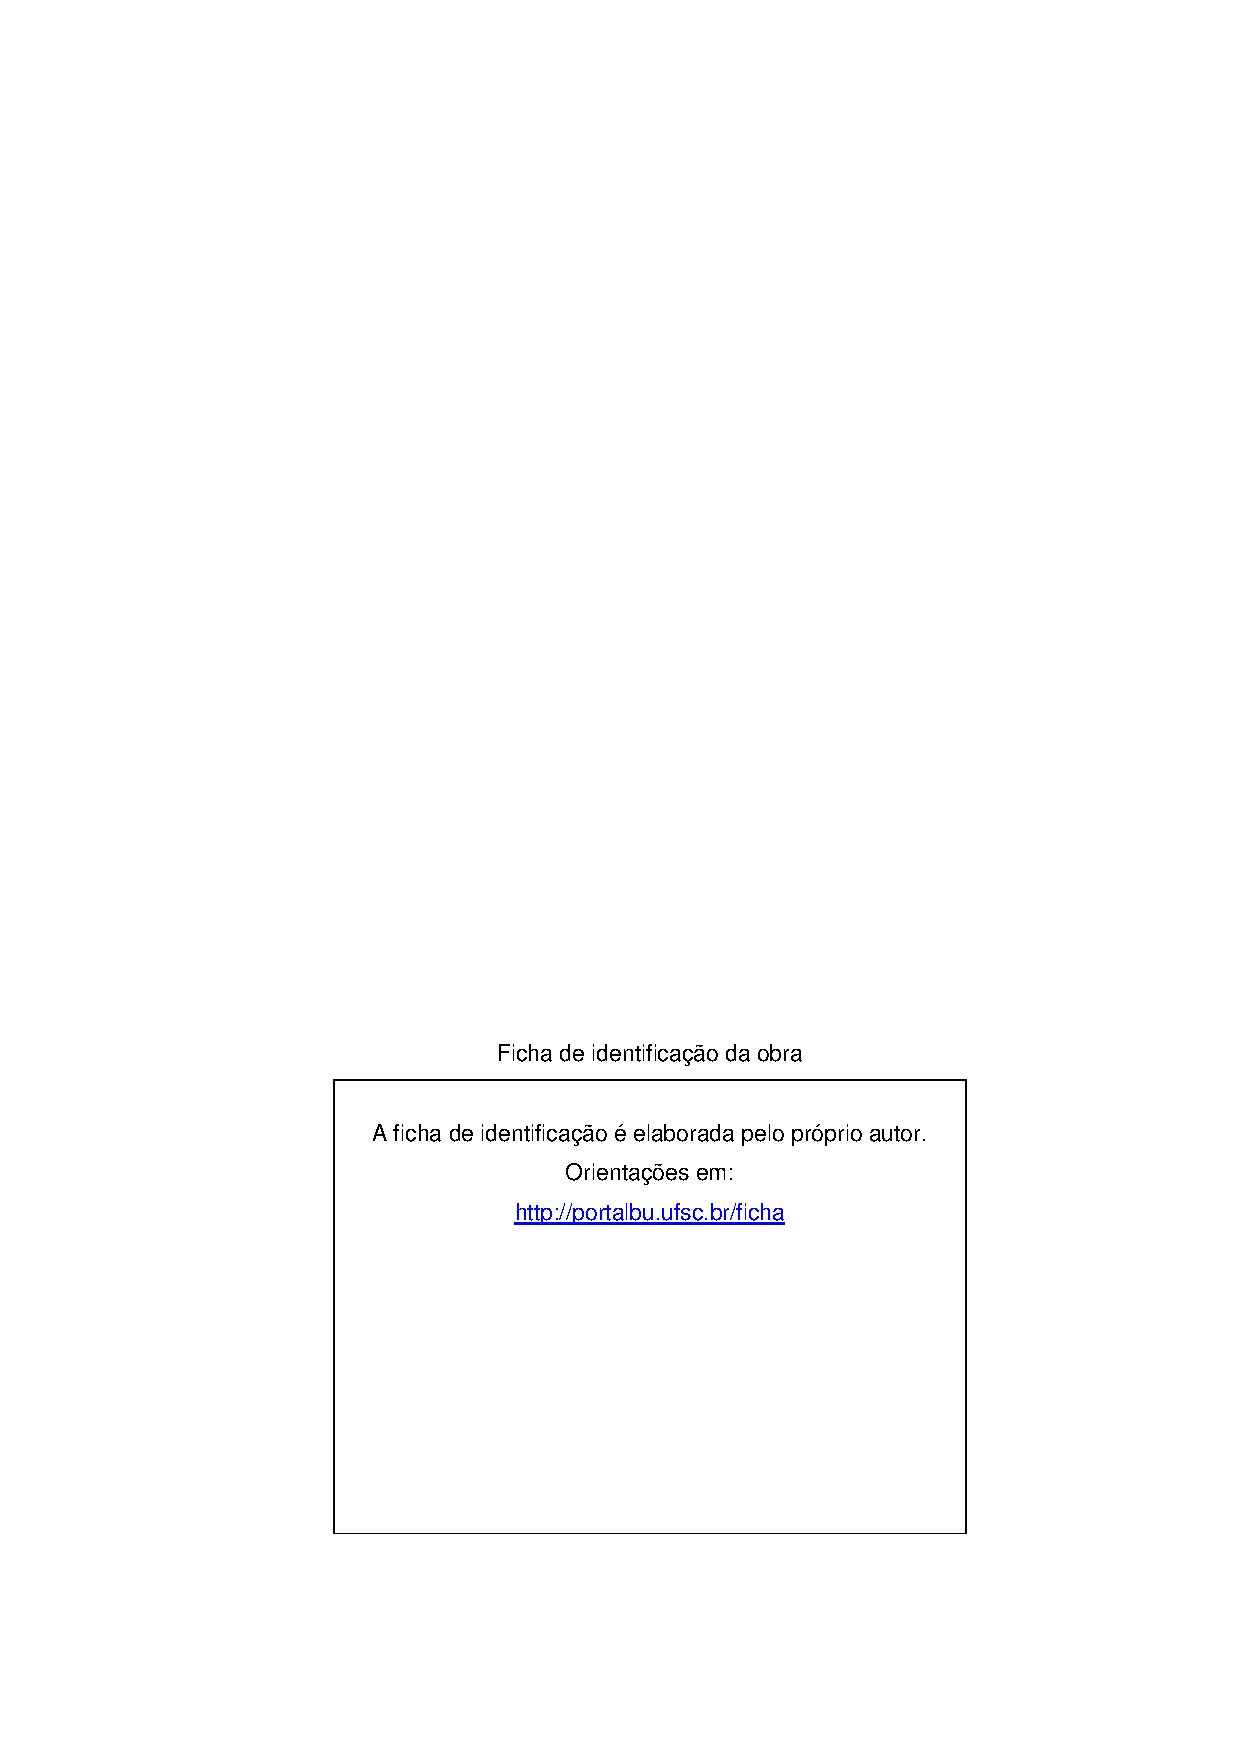
\includepdf{pictures/Ficha_Catalografica.pdf}
    \ifforcedinclude\else\cleardoublepage\fi
\fi


% Inserir errata

% Inserir folha de aprovação. Isto é um exemplo de Folha de aprovação, elemento obrigatório da
% NBR 14724/2011 (seção 4.2.1.3). Você pode utilizar este modelo até a aprovação do trabalho.
% Após isso, substitua todo o conteúdo deste arquivo por uma imagem da página assinada pela
% banca com o comando abaixo:
\ifforcedinclude\else\cleardoublepage\fi


% \addtotextpreliminarycontent{\lang{Approval Sheet}{Folha de Aprovação}}

% \begin{folhadeaprovacao}

%   \begin{center}
%     {\imprimirautor}

%     \begin{center}
%       \ABNTEXchapterfont\bfseries\MakeUppercase{\imprimirtitulo}\ifnotempty{\imprimirsubtitulo}{: \imprimirsubtitulo}
%     \end{center}

%     \begin{minipage}{\textwidth}
%       \lang
%       {
%         This \imprimirtipotrabalho~was considered appropriate to get the \imprimirformacao,
%         \ifnotempty{\imprimirarea}{in the area of \imprimirarea,}
%         and it was approved by the \imprimirprograma~of \imprimircentro~of \imprimirinstituicao.
%       }
%       {
%         Este(a) \imprimirtipotrabalho~foi julgado adequado(a) para obtenção do Título de \imprimirformacao,
%         \ifnotempty{\imprimirarea}{na área de concentração de \imprimirarea,}
%         e foi aprovado em sua forma final pelo \imprimirprograma~
%         do \imprimircentro~da \imprimirinstituicao.
%       }
%     \end{minipage}%
%   \end{center}

%   \begin{center}
%     \imprimirlocal, \imprimirdata.
%   \end{center}

%   \assinatura{%
%     \textbf{\imprimircoordenador} \\
%     \imprimircoordenadorRotulo~\lang{of}{do} \imprimirprograma
%   }

%   % \newpage
%   \begin{flushleft}
%     \textbf{\lang{Examination Board}{Banca Examinadora}:}
%   \end{flushleft}

%   \assinatura{%
%     \textbf{\imprimirorientador} \\ \imprimirorientadorRotulo\\
%     \imprimirinstituicao~--~\imprimirinstituicaosigla
%   }

%   \ifnotempty{\imprimircoorientador}{%
%     \assinatura{%
%       \textbf{\imprimircoorientador} \\ \imprimircoorientadorRotulo \\
%       \imprimirinstituicao~--~\imprimirinstituicaosigla
%     }
%   }

%   \assinatura{%
%     \textbf{Prof. Convidado 1, \lang{PhD.}{Dr.}} \\
%     Instituição 1 -- Sigla 1
%   }

%   \assinatura{%
%     \textbf{Prof. Convidado 2, \lang{PhD.}{Dr.}} \\
%     Instituição 2 -- Sigla 2
%   }

%   \assinatura{%
%     \textbf{Prof. Convidado 3, \lang{PhD.}{Dr.}} \\
%     Instituição 3 -- Sigla 3
%   }

%   \assinatura{%
%     \textbf{Prof. Convidado 4, \lang{PhD.}{Dr.}} \\
%     Instituição 4 -- Sigla 4
%   }

% \end{folhadeaprovacao}

\addtotextpreliminarycontent{\lang{Approval Sheet}{Folha de Aprovação}}

\begin{folhadeaprovacao}
  \OnehalfSpacing
  \centering
  \begin{center}
    {\imprimirautor}

    \begin{center}
      \ABNTEXchapterfont\bfseries\MakeUppercase{\imprimirtitulo}\ifnotempty{\imprimirsubtitulo}{: \imprimirsubtitulo}
    \end{center}

    \begin{minipage}{\textwidth}
      \begin{center}
        \lang
        {
          % This \imprimirtipotrabalho~was considered appropriate to get the \imprimirformacao,
          % \ifnotempty{\imprimirarea}{in the area of \imprimirarea,}
          % and it was approved by the \imprimirprograma~of \imprimircentro~of \imprimirinstituicao.
          The present \imprimirnivel~thesis was evaluated and approved by examination board formed
          by the following members:\\
        }
        {
          % Este(a) \imprimirtipotrabalho~foi julgado adequado(a) para obtenção do Título de \imprimirformacao,
          % \ifnotempty{\imprimirarea}{na área de concentração de \imprimirarea,}
          % e foi aprovado em sua forma final pelo \imprimirprograma~
          % do \imprimircentro~da \imprimirinstituicao.
          O presente trabalho em nível de \imprimirnivel~foi avaliado e
          aprovado por banca examinadora composta pelos seguintes membros:\\
        }
      \end{center}
    \end{minipage}%

    \vspace*{\baselineskip}
    \textbf{Prof. Convidado 1, \lang{PhD.}{Dr.}} \\
    Instituição 1 -- Sigla 1

    \vspace*{\baselineskip}
    \textbf{Prof. Convidado 2, \lang{PhD.}{Dr.}} \\
    Instituição 2 -- Sigla 2

    \vspace*{\baselineskip}
    \textbf{Prof. Convidado 3, \lang{PhD.}{Dr.}} \\
    Instituição 3 -- Sigla 3

    \vspace*{2\baselineskip}
    \begin{minipage}{\textwidth}
      \lang
      {
        We certify that this is the \textbf{original and final} version of this work, that was considered appropriate to get the \imprimirformacao.\\
      }
      {
        Certificamos que esta é a \textbf{versão original e final} deste trabalho, que foi julgado adequado para obtenção do título de \imprimirformacao.\\
      }
    \end{minipage}
    %    \vspace{-0.7cm}
    \vspace*{\fill}
    \assinatura{
      \OnehalfSpacing
      \textbf{\imprimircoordenador}
      \lang
      {
        Coordinator of the
      }
      {
        Coordenação do
      }
      \imprimirprograma

    }

    \vspace*{\fill}
    \assinatura{
      \OnehalfSpacing
      \textbf{\imprimirorientador} \\
      \imprimirorientadorRotulo
    }
    %	\ifnotempty{\imprimircoorientador}{
    %	\assinatura{\imprimircoorientador \\ \imprimircoorientadorRotulo \\
    %		\imprimirinstituicao~--~\imprimirinstituicaosigla}
    %	}
    % \newpage
    \vspace*{\fill}
    \imprimirlocal, \imprimirano.
  \end{center}


\end{folhadeaprovacao}
% \includepdf{pictures/folhadeaprovacao_final.pdf}


% Dedicatória
\ifforcedinclude\else\cleardoublepage\fi
\ifforcedinclude\else

\addtotextpreliminarycontent{\lang{Dedicatory}{Dedicatória}}

\begin{dedicatoria}

  \vspace*{\fill}
  \centering
  \noindent
  \textit{\lang
    {
      This work is dedicated to my grandmother Dulce Maria, \\
      and to my mother, Dulce A. Borges.
    }
    {
      Este trabalho é dedicado à minha avó Dulce Maria \\
      e à minha mãe, Dulce A. Borges..
    }
    % {
    %   This work is dedicated to adult children who, \\
    %   When small, dreamed of becoming scientists.
    % }
    % {
    %   Este trabalho é dedicado às crianças adultas que,\\
    %   quando pequenas, sonharam em se tornar cientistas.
    % }
  }
  \vspace*{\fill}

\end{dedicatoria}


\fi

% Agradecimentos
\ifforcedinclude\else\cleardoublepage\fi


\addtotextpreliminarycontent{\lang{Acknowledgement}{Agradecimentos}}

\begin{agradecimentos}

\lang
{
    Greetings.
}
{
    Os agradecimentos principais são direcionados à Gerald Weber, Miguel Frasson,
    Leslie H. Watter, Bruno Parente Lima, Flávio de Vasconcellos Corrêa, Otavio Real
    Salvador, Renato Machnievscz\footnote{Os nomes dos integrantes do primeiro
    projeto abn\TeX\ foram extraídos de
    \url{http://codigolivre.org.br/projects/abntex/}} e todos aqueles que
    contribuíram para que a produção de trabalhos acadêmicos conforme
    as normas ABNT com \LaTeX{} fosse possível.

    Agradecimentos especiais são direcionados ao Centro de Pesquisa em Arquitetura
    da Informação\footnote{\url{http://www.cpai.unb.br/}} da Universidade de
    Brasília (CPAI), ao grupo de usuários
    \emph{latex-br}\footnote{\url{http://groups.google.com/group/latex-br}} e aos
    novos voluntários do grupo
    \emph{\abnTeX{}}\footnote{\url{http://groups.google.com/group/abntex2} e
    \url{http://abntex2.googlecode.com/}}~que contribuíram e que ainda
    contribuirão para a evolução do \abnTeX{}.
}

\end{agradecimentos}


%Mesmo padrão da seção primária, porém sem indicativo numérico. Assim como: Dedicatória, Resumo, Abstract, Sumário, Listas, Referências, Apêndices e Anexos.
%
%
%Corpo do texto, fonte 10,5, justificado, recuo especial da primeira linha de 1 cm, espaçamento simples.
%


% Epígrafe
\ifforcedinclude\else\cleardoublepage\fi


\addtotextpreliminarycontent{\lang{Epigraph}{Epigrafe}}

\begin{epigrafe}

\vspace*{\fill}\lang
{
    \begin{flushright}
        \textit{``Learn from yesterday, live for today, hope for tomorrow. The important thing is not to stop questioning.''} \\ Albert Einstein
    \end{flushright}
    \begin{flushright}
        \textit{``The true sign of intelligence is not knowledge but imagination.''} \\  Albert Einstein
    \end{flushright}
    \begin{flushright}
        \textit{``Peace cannot be kept by force; it can only be achieved by understanding.''} \\ Albert Einstein
    \end{flushright}
    \begin{flushright}
        \textit{``Whoever is careless with the truth in small matters cannot be trusted with important matters.''} \\ Albert Einstein
    \end{flushright}
    \begin{flushright}
        \textit{``Extraordinary claims require extraordinary evidence''} \\ Carl Sagan
    \end{flushright}
    \begin{flushright}
        \textit{``Catholic, which I was until I reached the age of reason.''} \\ George Carlin
    \end{flushright}
    \begin{flushright}
        \textit{``We made too many wrong mistakes.''} \\ Yogi Berra
    \end{flushright}
}
{
    \begin{flushright}
        \textit{``Assim como aquele pecado da juventude, este documento te perseguirá pelo resto da vida.''} \\ Enio Valmor Kassick
    \end{flushright}
    \begin{flushright}
        \textit{``Estupidez trará mais autoconfiança do que o conhecimento e a bravura juntas. \englishword{\showfont}''} \\ Adriano Ruseler
    \end{flushright}
}

\end{epigrafe}





% Ajusta o espaçamento dos parágrafos do resumo
\setlength{\absparsep}{18pt}

% RESUMOS
\ifforcedinclude\else\cleardoublepage\fi


\newcommand{\imprimirbrazilabstract}{%
  \cleardoublepage\phantomsection
  \addtotextpreliminarycontent{Resumo em Português}
  \begin{otherlanguage*}{brazil}
    \begin{resumo}[Resumo]

      % Segundo a \textcite[3.1-3.2]{NBR6028:2003}, o resumo deve ressaltar o
      % objetivo, o método, os resultados e as conclusões do documento. A ordem e a extensão
      % destes itens dependem do tipo de resumo (informativo ou indicativo) e do
      % tratamento que cada item recebe no documento original. O resumo deve ser
      % precedido da referência do documento, com exceção do resumo inserido no
      % próprio documento. (\ldots) As palavras-chave devem figurar logo abaixo do
      % resumo, antecedidas da expressão Palavras-chave:, separadas entre si por
      % ponto e finalizadas também por ponto.

      % Além disso, na UFSC o texto do resumo deve ser digitado, em um único bloco, sem espaço de parágrafo. O resumo deve
      % ser significativo, composto de uma sequência de frases concisas, afirmativas e não de uma
      % enumeração de tópicos. Não deve conter citações. Deve usar o verbo na voz passiva. Abaixo do
      % resumo, deve-se informar as palavras-chave (palavras ou expressões significativas retiradas do
      % texto) ou, termos retirados de thesaurus da área. \englishword{\showfont}

      Deposição por energia direcionada a laser (L-DED), utilizando pó como material de adição, é uma tecnologia
      emergente na área de fabricação avançada, apresentando diversas características atraentes quando comparadas a
      outras técnicas de fabricação por manufatura aditiva de metais. Seu potencial para preencher as lacunas entre as etapas de
      desenvolvimento de produtos, prototipagem e produção de partes altamente otimizadas são notáveis, mas a complexidade
      inerente ao processo ainda levanta questionamentos relevantes que precisam ser abordados. Apesar de que
      a geometria de seções transversais de cordões individuais e paredes finas, bem como os efeitos dos parâmetros
      de processo na microestrutura resultante são amplamente discutidos na literatura para diferentes
      combinações de parâmetros e materiais processados, apenas alguns estudos investigam a formação de peças
      com características geométricas relevantes para produtos. Como o objetivo principal do processo é geralmente entregar
      componentes de boa qualidade, e a geometria final do componente desempenha um papel importante na definição de qualidade,
      o presente trabalho documenta uma abordagem inversa, investigando como características geométricas do componente
      afetam a geometria depositada resultante, para um determinado conjunto de parâmetros de processo. A espessura
      da parede, ângulo de inclinação e raio de curvatura de uma geometria paramétrica são manipulados para um
      conjunto de parâmetros de processo e as geometrias finais resultantes, bem como seções transversais locais
      são analisadas.

      \imprimirpalavraschave{Palavras-chaves}{\begin{inparaitem}[]\palavraschaveportugues\end{inparaitem}}

    \end{resumo}
  \end{otherlanguage*}
}


\newcommand{\imprimirenglishabstract}{%
  % https://tex.stackexchange.com/questions/20987/changing-babel-package-inside-a-single-chapter
  % https://tex.stackexchange.com/questions/36526/multiple-language-document-babel-selectlanguage-vs-begin-endotherlanguage
  \cleardoublepage\phantomsection
  \addtotextpreliminarycontent{English's Abstract}
  \begin{otherlanguage*}{english}
    \begin{resumo}[Abstract]

      Powder fed Laser Directed Energy Deposition (L-DED) is an emerging technology in the field
      of additive manufacturing, accounting for a variety of attractive features when compared to
      other metal additive manufacturing techniques. Its potential to fill the gaps between product
      development, prototyping and production of highly optimized parts are remarkable, but the inherent
      complexity of the process still raises relevant questions that need to be addressed. Although
      the cross-section geometry of single beads and thin walls, as well as the effects of process
      parameters on the resulting microstructure is widely discussed in the literature for different
      combinations of process parameters and materials, only a few studies investigate how bulk parts
      with product-like features are formed. As the main goal of the process is usually to deliver
      good quality parts, and the overall geometry plays a major role in the definition of quality,
      the present work takes an inverse approach, investigating how geometric features of the desired
      part affects the resulting deposited geometry, for a given set of process parameters. The wall
      thickness, draft angle and curvature radius of a benchmark geometry are manipulated for a fixed
      set of process parameters, and the resulting overall geometries, as well as local cross-sections
      are compared.

      \imprimirpalavraschave{Keywords}{\begin{inparaitem}[]\palavraschaveingles\end{inparaitem}}

    \end{resumo}
  \end{otherlanguage*}
}


% \newcommand{\imprimirfrenchabstract}{%
%     \addtotextpreliminarycontent{Français Résumé}
%     \begin{resumo}[Résumé]
%       \begin{otherlanguage*}{french}
%           Il s'agit d'un résumé en français.

%           \imprimirpalavraschave{Mots-clés}{latex. abntex. publication de textes.}
%       \end{otherlanguage*}
%     \end{resumo}
% }


% \newcommand{\imprimirspanishabstract}{%
%     \addtotextpreliminarycontent{Español Resumen}
%     \begin{resumo}[Resumen]
%       \begin{otherlanguage*}{spanish}
%           Este es el resumen en español.

%           \imprimirpalavraschave{Palabras clave}{latex. abntex. publicación de textos.}
%       \end{otherlanguage*}
%     \end{resumo}
% }


\makeatletter
\ifenglish
  \@ifundefined{imprimirbrazilabstract}{}{\imprimirbrazilabstract}

  % % https://tex.stackexchange.com/questions/331108/times-new-roman-in-latex-just-some-text
  % % https://tex.stackexchange.com/questions/11707/how-to-force-output-to-a-left-or-right-page
  % % https://tex.stackexchange.com/questions/132966/do-not-display-chapter-title-in-memoir-class
  % \cleardoublepage\phantomsection
  % \pretextualchapter{Resumo Expandido}
  % \addtotextpreliminarycontent{Resumo Expandido}

  % \begin{otherlanguage*}{brazil}
  %   \setlength{\parskip}{0.2cm}
  %   \setlength{\parindent}{0.0cm}
  %   \fontfamily{ptm}\selectfont

  %   \section*{Introdução}
  %   O resumo expandido é previsto na Resolução Normativa nº 95/CUn/2017, Art. 55, § 2, de 4 de
  %   abril de 2017, e exigido para teses e dissertações escritas em idiomas estrangeiros (com
  %   exceção dos cursos pertinentes ao estudo de idiomas estrangeiros – Programa de Pós-Graduação
  %   em Estudos da Tradução e Programa de Pós-Graduação em Inglês: Estudos Linguísticos e
  %   Literários).

  %   O resumo expandido é considerado um elemento pré-textual e deverá ser incluído no trabalho
  %   após o resumo e antes do abstract. Deverá iniciar em página impar (no anverso de uma folha)
  %   continuando no verso da folha. O texto deverá seguir o formato A5, com margens espelhadas:
  %   superior 2,0 cm, inferior 1,5 cm, interna 2,5 cm e externa 1,5. Deve ser empregada a fonte
  %   Time New Roman.  Todo o texto deve ser digitado em tamanho 10,5. O espaçamento entre as
  %   linhas deverá ser simples. A expressão “resumo expandido” deve seguir a mesma tipografia das
  %   demais sessões primárias do trabalho.

  %   O texto do resumo expandido deve ser redigido em português e conter as seguintes seções (ver
  %   modelo): Introdução, Objetivos, Metodologia, Resultados e Discussão e Considerações Finais.
  %   Deve apresentar no mínimo duas (02) e, no máximo, cinco (05) páginas contendo a mesma
  %   formatação em A5 do resumo e do abstract, bem como palavras-chave. \englishword{\showfont}

  %   \section*{Objetivos}
  %   Lorem ipsum dolor sit amet, consectetur adipiscing elit. Phasellus vitae dolor lacus. Ut
  %   accumsan vitae felis nec porttitor. Integer interdum fringilla feugiat. Nullam pulvinar sit
  %   amet tellus eget maximus. Donec sit amet magna eget justo semper fermentum vel eget velit.
  %   In iaculis imperdiet mauris, ac ornare libero placerat non. Nulla libero lectus, ullamcorper
  %   ac ornare eget, pulvinar ac nulla. Curabitur vestibulum non nisl eget sagittis. Proin
  %   gravida lacus id eros bibendum interdum. Mauris ullamcorper elementum tortor sed consequat.
  %   Integer tempus, est a lobortis vehicula, nisi mi fringilla augue, non semper leo metus in
  %   quam. Etiam in leo maximus, pulvinar mi eget, vehicula risus. Donec sed dui semper, dictum
  %   eros at, suscipit felis.

  %   Nam sagittis vel orci at tempus. Nulla non pellentesque eros.
  %   Quisque cursus leo massa, eu ultricies nisl lacinia a. Nulla sit amet elementum ligula.
  %   Proin sodales venenatis dictum. Ut et est cursus, vulputate velit et, viverra odio. Interdum
  %   et malesuada fames ac ante ipsum primis in faucibus. Maecenas purus diam, tempor a semper
  %   et, finibus a ex. Cras sagittis felis urna, et consequat arcu lacinia ut. Praesent blandit
  %   venenatis ante nec porta. Duis rutrum, tellus vitae ullamcorper auctor, lectus ex laoreet
  %   est, ac tristique ipsum arcu vitae nibh. Nam efficitur felis ut mi consectetur, nec auctor
  %   odio ornare. In tempor vulputate urna, vitae cursus enim egestas eu. Proin diam augue,
  %   dignissim vitae ligula eget, lobortis ornare odio. Duis quis elit augue. Fusce quis rhoncus
  %   tortor. Donec hendrerit at massa a mattis. Sed ipsum neque, aliquam ut sem sed, ultrices
  %   varius ligula. Suspendisse blandit, dolor ac rhoncus lacinia, dolor purus cursus purus, et
  %   accumsan orci neque a leo.

  %   \section*{Metodologia}
  %   Quisque efficitur dolor in lectus dapibus elementum. Nam ultrices blandit consectetur.
  %   Nullam ultricies sit amet odio quis placerat. Aenean eget est elit. Maecenas et nulla dolor.
  %   Orci varius natoque penatibus et magnis dis parturient montes, nascetur ridiculus mus. In
  %   pulvinar velit sed mi sagittis ornare. Aenean rutrum suscipit egestas. Phasellus pharetra
  %   eget ex in volutpat. Quisque eu arcu nunc. Vivamus arcu ligula, pharetra at rhoncus sit
  %   amet, pulvinar sed eros. Sed porta ipsum ipsum, et fermentum magna volutpat sed. Vivamus
  %   pharetra facilisis orci, sit amet luctus nisl pretium id. Sed consequat, arcu et congue
  %   pulvinar, risus enim aliquet purus, eget venenatis libero leo sit amet metus. Maecenas vitae
  %   elit sapien. Fusce mollis libero et gravida placerat. Proin ut quam quis justo aliquam
  %   dictum. Donec volutpat convallis suscipit. Vivamus metus nisl, placerat ac enim vitae,
  %   tempus ultricies odio.

  %   Aliquam ac vehicula arcu, non bibendum nulla. Morbi libero sem,
  %   imperdiet vel quam et, posuere tempus nunc. Maecenas dictum magna sit amet ligula facilisis
  %   commodo. Aliquam tellus diam, ornare vel elementum in, dignissim id purus. Ut at tortor non
  %   sem molestie euismod non at turpis. Phasellus vitae bibendum tellus. Suspendisse odio enim,
  %   faucibus eget congue quis, semper sit amet tortor. Sed ac lectus est. Pellentesque nec
  %   mattis mi, et varius dolor. Aliquam quis massa ac tellus malesuada sollicitudin. Maecenas
  %   ultrices risus massa, nec auctor risus sagittis id. Praesent a sapien nulla. Donec
  %   tincidunt, metus quis hendrerit facilisis, enim augue convallis elit, sed consequat lacus
  %   odio vitae magna.

  %   \section*{Resultados e Discussão}
  %   Nullam sed cursus leo. Donec commodo volutpat hendrerit. Fusce et tempus lectus, feugiat
  %   consequat est. Class aptent taciti sociosqu ad litora torquent per conubia nostra, per
  %   inceptos himenaeos. Nam quis cursus mauris, non tempus orci. Phasellus lobortis et mauris at
  %   vulputate. Sed nec nisl elementum lorem commodo gravida non a enim. Phasellus neque erat,
  %   aliquet ac ligula ac, maximus vestibulum sem. Vestibulum vel tincidunt turpis. Donec lacinia
  %   rutrum dolor dapibus bibendum. Mauris pharetra nibh nec tincidunt iaculis. Vivamus pharetra
  %   bibendum nisl eget blandit. In lobortis diam non justo eleifend, id lobortis ante fringilla.
  %   Donec libero tortor, suscipit vestibulum vestibulum id, rutrum accumsan turpis. Phasellus
  %   sollicitudin luctus tincidunt. Suspendisse potenti. Nam semper metus et mi pharetra, in
  %   pretium ligula fermentum. Integer consectetur, orci non placerat feugiat, dui ex gravida
  %   augue, vel placerat ligula augue vel velit. Aliquam sollicitudin pellentesque congue. Donec
  %   vitae turpis in ante posuere posuere. Pellentesque eu justo leo. Donec quis elit vitae leo
  %   varius luctus quis eget justo.

  %   Vestibulum elementum ex neque, quis commodo tortor porttitor
  %   mattis. Mauris vel sagittis turpis. Aenean ligula turpis, eleifend at felis sed, cursus
  %   condimentum orci. Fusce accumsan est odio, eu venenatis massa sodales in. Curabitur a tempor
  %   nisl. Quisque consequat sed arcu a congue. In viverra, ex ut hendrerit condimentum, urna sem
  %   euismod eros, nec suscipit turpis dolor eget augue. Aenean posuere tellus et consectetur
  %   condimentum. Mauris et massa et nulla fringilla interdum. Duis quis posuere elit. Donec at
  %   ex non arcu faucibus rutrum et vel lectus. Vivamus pellentesque vestibulum rutrum. Sed
  %   pretium, purus sed efficitur feugiat, nisi justo eleifend nibh, id suscipit nunc massa nec
  %   lectus. In euismod enim eu sapien dictum sodales. Fusce sit amet vulputate orci. Nulla
  %   rutrum mauris at purus aliquet, ac sollicitudin leo laoreet. Etiam elementum posuere
  %   feugiat. Maecenas sed libero non augue fermentum ultricies eget at mi. Aenean auctor
  %   bibendum lacus, dignissim aliquet est tempus eget. Maecenas tempus, nulla id rhoncus
  %   suscipit, augue leo auctor mi, eget tincidunt magna mi quis dui. Maecenas ut elit in turpis
  %   tincidunt ultrices. Nulla id nulla aliquet, porttitor eros quis, egestas justo. Nunc nisi
  %   quam, egestas a accumsan fermentum, ultricies ac elit.

  %   Nulla porta auctor vestibulum. Sed
  %   consectetur lacus molestie iaculis ullamcorper. Proin porta posuere massa a lacinia. Nunc a
  %   lacinia orci, non vehicula ante. Vestibulum ipsum velit, congue et neque aliquam, imperdiet
  %   ornare augue. Donec et congue sapien. Pellentesque consequat consectetur neque ut varius. In
  %   aliquam ex quis ante venenatis dapibus. Vivamus et imperdiet urna. Vestibulum quis nibh
  %   magna. In a congue lectus, eu sodales nunc. Suspendisse id.

  %   \section*{Considerações Finais}
  %   Lorem ipsum dolor sit amet, consectetur adipiscing elit. Phasellus vitae dolor lacus. Ut
  %   accumsan vitae felis nec porttitor. Integer interdum fringilla feugiat. Nullam pulvinar sit
  %   amet tellus eget maximus. Donec sit amet magna eget justo semper fermentum vel eget velit.
  %   In iaculis imperdiet mauris, ac ornare libero placerat non. Nulla libero lectus, ullamcorper
  %   ac ornare eget, pulvinar ac nulla. Curabitur vestibulum non nisl eget sagittis. Proin
  %   gravida lacus id eros bibendum interdum. Mauris ullamcorper elementum tortor sed consequat.
  %   Integer tempus, est a lobortis vehicula, nisi mi fringilla augue, non semper leo metus in
  %   quam. Etiam in leo maximus, pulvinar mi eget, vehicula risus. Donec sed dui semper, dictum
  %   eros at, suscipit felis.

  %   Nam sagittis vel orci at tempus. Nulla non pellentesque eros.
  %   Quisque cursus leo massa, eu ultricies nisl lacinia a. Nulla sit amet elementum ligula.
  %   Proin sodales venenatis dictum. Ut et est cursus, vulputate velit et, viverra odio. Interdum
  %   et malesuada fames ac ante ipsum primis in faucibus. Maecenas purus diam, tempor a semper
  %   et, finibus a ex. Cras sagittis felis urna, et consequat arcu lacinia ut. Praesent blandit
  %   venenatis ante nec porta. Duis rutrum, tellus vitae ullamcorper auctor, lectus ex laoreet
  %   est, ac tristique ipsum arcu vitae nibh. Nam efficitur felis ut mi consectetur, nec auctor
  %   odio ornare. In tempor vulputate urna, vitae cursus enim egestas eu. Proin diam augue,
  %   dignissim vitae ligula eget, lobortis ornare odio. Duis quis elit augue. Fusce quis rhoncus
  %   tortor. Donec hendrerit at massa a mattis. Sed ipsum neque, aliquam ut sem sed, ultrices
  %   varius ligula. Suspendisse blandit, dolor ac rhoncus lacinia, dolor purus cursus purus, et
  %   accumsan orci neque a leo.


  %   \imprimirpalavraschave{Palavras-chaves}{\begin{inparaitem}[]\palavraschaveportugues\end{inparaitem}}

  % \end{otherlanguage*}

  \@ifundefined{imprimirenglishabstract}{}{\imprimirenglishabstract}

\else
  \@ifundefined{imprimirbrazilabstract}{}{\imprimirbrazilabstract}
  \@ifundefined{imprimirenglishabstract}{}{\imprimirenglishabstract}
\fi

\@ifundefined{imprimirfrenchabstract}{}{\imprimirfrenchabstract}
\@ifundefined{imprimirspanishabstract}{}{\imprimirspanishabstract}
\makeatother



% Some tables of contents
\ifforcedinclude\else
{
    % https://tex.stackexchange.com/questions/179506/disable-colorlinks-locally-or-just-for-the-toc
    \hypersetup{hidelinks}

    % inserir lista de figuras
    \ifforcedinclude\else\cleardoublepage\fi
    % https://tex.stackexchange.com/questions/234398/list-of-figures-and-tables-when-there-are-no-figures-or-tables
    \whenlistisnotempty{\listfigurename}{%
        \addtotextpreliminarycontent{\listfigurename}
        % https://tex.stackexchange.com/questions/121879/remove-spacing-between-per-chapter-figures-in-lof
        {\renewcommand{\addvspace}[1]{}
        \listoffigures*}
    }{\pdfbookmark[0]{\listfigurename}{lof}}

    % inserir lista de quadros
    \ifforcedinclude\else\cleardoublepage\fi
    % https://tex.stackexchange.com/questions/234398/list-of-figures-and-tables-when-there-are-no-figures-or-tables
    \whenlistisnotempty{\listofquadrosname}{%
        \addtotextpreliminarycontent{\listofquadrosname}
        % https://tex.stackexchange.com/questions/121879/remove-spacing-between-per-chapter-figures-in-lof
        {\renewcommand{\addvspace}[1]{}
        \listofquadros*}
    }{\pdfbookmark[0]{\listofquadrosname}{loq}}

    % inserir lista de tabelas
    \ifforcedinclude\else\cleardoublepage\fi
    % https://tex.stackexchange.com/questions/234398/list-of-figures-and-tables-when-there-are-no-figures-or-tables
    \whenlistisnotempty{\listtablename}{%
        \addtotextpreliminarycontent{\listtablename}
        % https://tex.stackexchange.com/questions/121879/remove-spacing-between-per-chapter-figures-in-lof
        {\renewcommand{\addvspace}[1]{}
        \listoftables*}
    }{\pdfbookmark[0]{\listtablename}{lot}}

    % inserir códigos fonte (List of Listings `lol`)
    % https://tex.stackexchange.com/questions/511519/latex-keeps-showing-minted-environment-as-figures-instead-of-listening/511579#511579
    \ifforcedinclude\else\cleardoublepage\fi
    % https://tex.stackexchange.com/questions/234398/list-of-figures-and-tables-when-there-are-no-figures-or-tables
    \whenlistisnotempty{\lstlistlistingname}{%
        \addtotextpreliminarycontent{\lstlistlistingname}
        % https://tex.stackexchange.com/questions/121879/remove-spacing-between-per-chapter-figures-in-lof
        {\renewcommand{\addvspace}[1]{}
        \lstlistoflistings*}
    }{\pdfbookmark[0]{\lstlistlistingname}{lol}}
}
\fi


% inserir lista de abreviaturas e siglas
\ifforcedinclude\else\cleardoublepage\fi


\addtotextpreliminarycontent{\lang{List of Acronyms}{Lista de Siglas}}

\begin{siglas}
    \item[ABNT] \lang{Brazilian Association of Technical Standards}{Associação Brasileira de Normas Técnicas}
    \item[abnTeX] \lang{Absurd Standards for TeX}{ABsurdas Normas para TeX}
\end{siglas}



% Inserir lista de símbolos
\ifforcedinclude\else\cleardoublepage\fi


\addtotextpreliminarycontent{\lang{List of Symbols}{Lista de Símbolos}}

% Devam aparecer na mesma ordem de ocorrência no texto.
\begin{simbolos}
    \item[$ \Gamma $] \lang{Greek letter Gama}{Letra grega Gama}
    \item[$ \Lambda $] \lang{Lambda}{Lambda}
    \item[$ \zeta $] \lang{Minimal Greek letter zeta}{Letra grega minúscula zeta}
    \item[$ \in $] \lang{Belongs}{Pertence}
\end{simbolos}


% How to remove the self-reference of the ToC from the ToC?
% https://tex.stackexchange.com/questions/10943/how-to-remove-the-self-reference-of-the-toc-from-the-toc
\ifforcedinclude\else\cleardoublepage\fi

\begin{KeepFromToc}
    % https://tex.stackexchange.com/questions/35/what-does-overfull-hbox-mean
    % https://tex.stackexchange.com/questions/59122/how-to-avoid-using-sloppy-document-wide-to-fix-overfull-hbox-problems
    % https://tex.stackexchange.com/questions/257007/adding-color-to-table-of-contents-and-section-headings
    {
        % https://tex.stackexchange.com/questions/179506/disable-colorlinks-locally-or-just-for-the-toc
        \hypersetup{hidelinks}

        % https://tex.stackexchange.com/questions/65711/underfull-vbox-badness-10000-with-memoir
        \raggedbottom

        % https://tex.stackexchange.com/questions/49887/overfull-hbox-warning-for-toc-entries-when-using-memoir-documentclass
        % \makeatletter
            % \renewcommand{\@pnumwidth}{2em}
            % \renewcommand{\@tocrmarg}{3em}
        % \makeatother

        % https://tex.stackexchange.com/questions/57544/memoir-mysterious-overfull-hbox-in-toc-when-mathptmx-is-used
        % \setlength{\cftchapternumwidth}{2.25em}

        % Add the table of contents to the brief table of contents
        % https://tex.stackexchange.com/questions/234398/list-of-figures-and-tables-when-there-are-no-figures-or-tables
        \whenlistisnotempty{\contentsname}{%
            \addtotextpreliminarycontent{\contentsname}
            \tableofcontents
        }{\pdfbookmark[0]{\contentsname}{toc}}
    }

\end{KeepFromToc}


% ---

% ----------------------------------------------------------
% ELEMENTOS TEXTUAIS
% ----------------------------------------------------------
\textual

% ---
% 1 - Introdução
% ---
% ----------------------------------------------------------
\chapter{Introdução}
% ----------------------------------------------------------

As orientações aqui apresentadas são baseadas em um conjunto de normas elaboradas pela \gls{ABNT}. Além das normas técnicas, a Biblioteca também elaborou uma série de tutoriais, guias, \textit{templates} os quais estão disponíveis em seu site, no endereço \url{http://portal.bu.ufsc.br/normalizacao/}.

Paralelamente ao uso deste \textit{template} recomenda-se que seja utilizado o \textbf{Tutorial de Trabalhos Acadêmicos} (disponível neste link \url{https://repositorio.ufsc.br/handle/123456789/180829}) e/ou que o discente \textbf{participe das capacitações oferecidas da Biblioteca Universitária da UFSC}.

Este \textit{template} está configurado apenas para a impressão utilizando o anverso das folhas, caso você queira imprimir usando a frente e o verso, acrescente a opção \textit{openright} e mude de \textit{oneside} para \textit{twoside} nas configurações da classe \textit{abntex2} no início do arquivo principal \textit{main.tex} \cite{abntex2classe}.

Conforme a \href{https://repositorio.ufsc.br/bitstream/handle/123456789/197121/RN46.2019.pdf?sequence=1&isAllowed=y}{Resolução NORMATIVA nº 46/2019/CPG} as dissertações e teses não serão mais entregues em formato impresso na Biblioteca Universitária. Consulte o Repositório Institucional da UFSC ou sua Secretaria de Pós Graduação sobre os procedimentos para a entrega. 

\nocite{NBR6023:2002}
\nocite{NBR6027:2012}
\nocite{NBR6028:2003}
\nocite{NBR10520:2002}

% ----------------------------------------------------------
\section{Objetivos}
% ----------------------------------------------------------

Nas seções abaixo estão descritos o objetivo geral e os objetivos 
específicos.

% ----------------------------------------------------------
\subsection{Objetivo Geral}
% ----------------------------------------------------------

Descrição...

% ----------------------------------------------------------
\subsection{Objetivos Específicos}
% ----------------------------------------------------------

Descrição...
% ---

% ---
% 2 - Capítulo 2
% ---
% ----------------------------------------------------------
\chapter{Desenvolvimento}\label{cap:desenvolvimento}
% ----------------------------------------------------------
Deve-se inserir texto entre as seções.

% ----------------------------------------------------------
\section{Exposição do tema ou matéria}
% ----------------------------------------------------------

É a parte principal e mais extensa do trabalho. Deve apresentar a fundamentação teórica, a metodologia, os resultados e a discussão. Divide-se em seções e subseções conforme a NBR 6024 \cite{NBR6024:2012}.

Quanto à sua estrutura e projeto gráfico, segue as recomendações da \gls{ABNT} para preparação de trabalhos acadêmicos, a NBR 14724, de 2011 \cite{NBR14724:2011}.

\begin{figure}[htb]
	\caption{\label{fig:Fig_1}Elementos do trabalho acadêmico.}
	\begin{center}
		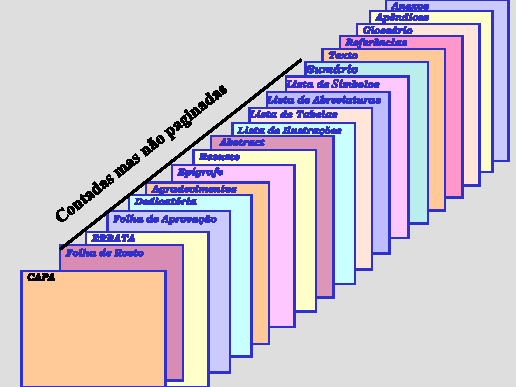
\includegraphics{images/imagem.pdf}
	\end{center}
	\fonte{Universidade Federal do Paraná (1996).}
\end{figure}

% ----------------------------------------------------------
\subsection{Formatação do texto}
% ----------------------------------------------------------

No que diz respeito à estrutura do trabalho, recomenda-se que:
\begin{alineas}
	\item o texto deve ser justificado, digitado em cor preta, podendo utilizar outras cores somente para as ilustrações;
	\item utilizar papel branco ou reciclado para impressão;
	\item os elementos pré-textuais devem iniciar no anverso da folha, com exceção da ficha catalográfica ou ficha de identificação da obra;
	\item os elementos textuais e pós-textuais devem ser digitados no anverso e verso das folhas, quando o trabalho for impresso. As seções primárias devem começar sempre em páginas ímpares, quando o trabalho for impresso. Deixar um espaço entre o título da seção/subseção e o texto e entre o texto e o título da subseção.
\end{alineas}

No \autoref{qua:Quadro_1} estão as especificações para a formatação do texto.

\begin{quadro}[htb]
	\centering
	\caption{\label{qua:Quadro_1}Formatação do texto.}	
	\begin{tabular}{|l|p{11cm}|}
		\hline
		\textbf{Formato do papel} & A4.\\ \hline
		\textbf{Impressão}        & A norma recomenda que caso seja necessário imprimir, deve-se utilizar a frente e o verso da página.\\ \hline
		\textbf{Margens}          & Superior: 3, Inferior: 2, Interna: 3 e Externa: 2. Usar margens espelhadas quando o  trabalho for impresso.\\ \hline
		\textbf{Paginação}        & As páginas dos elementos pré-textuais devem ser contadas, mas não numeradas. Para trabalhos digitados somente no anverso, a numeração das páginas deve constar no canto superior direito da página, a 2 cm da borda, figurando a partir da primeira folha da  parte textual. Para trabalhos digitados no anverso e no verso, a numeração deve constar no canto superior direito, no anverso, e no canto superior esquerdo no verso.\\ \hline
		\textbf{Espaçamento}      & O texto deve ser redigido com espaçamento entre linhas 1,5, excetuando-se as citações de mais de três linhas, notas de rodapé, referências, legendas das ilustrações e das tabelas, natureza (tipo do trabalho, objetivo, nome da instituição a que é submetido e área de concentração), que devem ser digitados em espaço simples, com fonte menor. As referências devem ser separadas entre si por um espaço simples em branco.\\ \hline
		\textbf{Paginação}        & A contagem inicia na folha de rosto, mas se insere o número da página na introdução até o final do trabalho.\\ \hline
		\textbf{Fontes sugeridas} & Arial ou Times New Roman.\\ \hline
		\textbf{Tamanho da fonte} & \textbf{Fonte tamanho 12 para o texto}, incluindo os títulos das seções e subseções. As citações com mais de três linhas, notas de rodapé, paginação, dados internacionais de catalogação, legendas e fontes das ilustrações e das tabelas devem ser de tamanho menor. Adotamos, neste \textit{template} \textbf{fonte tamanho 10}.\\ \hline
		\textbf{Nota de rodapé}   & Devem ser digitadas dentro da margem, ficando separadas por um espaço simples por entre as linhas e por filete de 5 cm a partir da margem esquerda. A partir da segunda linha, devem ser alinhadas embaixo da primeira letra da primeira palavra da primeira linha.\\ \hline
	\end{tabular}
	\fonte{\textcite{NBR14724:2011}.}
\end{quadro}

% ----------------------------------------------------------
\subsubsection{As ilustrações}
% ----------------------------------------------------------

Independentemente do tipo de ilustração (quadro, desenho, figura, fotografia, mapa, entre outros), a sua identificação aparece na parte superior, precedida da palavra designativa. 

\begin{citacao}
	Após a ilustração, na parte inferior, indicar a fonte consultada (elemento obrigatório, mesmo que seja produção do próprio autor), legenda, notas e outras informações necessárias à sua compreensão (se houver). A ilustração deve ser citada no texto e inserida o mais próximo possível do texto a que se refere. \cite[p. 11]{NBR14724:2011}.
\end{citacao}

% ----------------------------------------------------------
\subsubsection{Equações e fórmulas}
% ----------------------------------------------------------

As equações e fórmulas devem ser destacadas no texto para facilitar a leitura.  Para numerá-las, usar algarismos arábicos entre parênteses e alinhados à direita. Pode-se adotar uma entrelinha maior do que a usada no texto \cite{NBR14724:2011}.

Exemplos, \autoref{eq:Eq_1} e \autoref{eq:Eq_2}.

\begin{equation}\label{eq:Eq_1}
\gls{C} = 2 \gls{pi} \gls{r}
\end{equation}

\begin{equation}\label{eq:Eq_2}
\gls{A} = \gls{pi} \gls{r}^2
\end{equation}

% ----------------------------------------------------------
\subsubsubsection{Exemplo tabela}
% ----------------------------------------------------------

De acordo com \textcite{ibge1993}, tabela é uma forma não discursiva de apresentar informações em que os números representam a informação central. Ver \autoref{tab:Tab_1}.

\begin{table}[htb]
	\ABNTEXfontereduzida
	\caption{\label{tab:Tab_1}Médias concentrações urbanas 2010-2011.}
	\begin{tabular}{@{}p{3.0cm}p{1.5cm}p{2cm}p{2.5cm}p{2.5cm}p{2.5cm}@{}}
		\toprule
		\textbf{Média concentração urbana} & \multicolumn{2}{l}{\textbf{População}} & \textbf{Produto Interno Bruto – PIB (bilhões R\$)} & \textbf{Número de empresas} & \textbf{Número de unidades locais} \\ \midrule
		\textbf{Nome}                      & \textbf{Total}   & \textbf{No Brasil}  &                                                   &                             & \\
		Ji-Paraná (RO)                     & 116 610          & 116 610             & 1,686                                             & 2 734                       & 3 082 \\
		Parintins (AM)                     & 102 033          & 102 033             & 0,675                                             & 634                         & 683 \\
		Boa Vista (RR)                     & 298 215          & 298 215             & 4,823                                             & 4 852                       & 5 187 \\
		Bragança (PA)                      & 113 227          & 113 227             & 0,452                                             & 654                         & 686 \\ \bottomrule
	\end{tabular}
	\fonte{\textcite{ibge2016}.}
\end{table}
% ---

% ---
% 3 - Capítulo 3
% ---
% ----------------------------------------------------------
\chapter{Seção}
% ----------------------------------------------------------

Este \textit{template} contém algumas seções criadas na tentativa de facilitar seu uso. No entanto, não há um limite máximo ou mínimo de seção a ser utilizado no trabalho. Cabe a cada autor definir a quantidade que melhor atenda à sua 
necessidade.  
% ---

% ---
% 4 - Conclusão
% ---
%\phantompart
% ----------------------------------------------------------
\chapter{Conclusão}
% ----------------------------------------------------------

As conclusões devem responder às questões da pesquisa, em relação aos objetivos e às hipóteses. Devem ser breves, podendo apresentar recomendações e sugestões para trabalhos futuros.

% ----------------------------------------------------------
% ELEMENTOS PÓS-TEXTUAIS
% ----------------------------------------------------------
\postextual
% ----------------------------------------------------------

% ----------------------------------------------------------
% Referências bibliográficas
% ----------------------------------------------------------
\begingroup
\printbibliography[title=REFERÊNCIAS]
\endgroup

% ----------------------------------------------------------
% Glossário
% ----------------------------------------------------------
%
% Consulte o manual da classe abntex2 para orientações sobre o glossário.
%
%\glossary

% ----------------------------------------------------------
% Apêndices
% ----------------------------------------------------------

% ---
% Inicia os apêndices
% ---
\begin{apendicesenv}
	%	\partapendices* 
	% ----------------------------------------------------------
\chapter{Descrição 1}
% ----------------------------------------------------------

Textos elaborados pelo autor, a fim de completar a sua argumentação. Deve ser precedido da palavra APÊNDICE, identificada por letras maiúsculas consecutivas, travessão e pelo respectivo título. Utilizam-se letras maiúsculas dobradas quando esgotadas as letras do alfabeto. 

\end{apendicesenv}
% ---


% ----------------------------------------------------------
% Anexos
% ----------------------------------------------------------

% ---
% Inicia os anexos
% ---
\begin{anexosenv}
	%	\partanexos*
	% ----------------------------------------------------------
\chapter{Descrição 2}
% ----------------------------------------------------------

São documentos não elaborados pelo autor que servem como fundamentação (mapas, leis, estatutos). Deve ser precedido da palavra ANEXO, identificada por letras maiúsculas consecutivas, travessão e pelo respectivo título. Utilizam-se letras maiúsculas dobradas quando esgotadas as letras do alfabeto. 

\end{anexosenv}

%---------------------------------------------------------------------
% INDICE REMISSIVO
%---------------------------------------------------------------------
%\phantompart
%\printindex
%---------------------------------------------------------------------

\end{document}
